\documentclass[10pt,a4paper]{article}
\usepackage[utf8]{inputenc}
\usepackage[francais]{babel}
\usepackage[T1]{fontenc}
\usepackage{graphicx}
\usepackage[export]{adjustbox}
\author{Ali CHERIFI}
\title{Rapport de stage de licence\\Résumé vidéo et vidéo 3D anaglyphe et side-by-side}
\begin{document}
\maketitle
\newpage
\tableofcontents
\newpage
\section{Introduction}
Le relief de la vision humaine provient de la différence de perception entre les deux yeux. La stéréoscopie rassemble toutes les différentes méthodes permettant de reconstruire cet effet à partir d'objets 2D
observés soit à travers un instrument d'optique ou alors à partir de deux photographies prises avec un décalage.
La stéréoscopie est un domaine qui a interessé l'homme depuis longtemps. En effet, ce principe a été imaginé par Charles Wheatstone (physicien et inventeur anglais) en 1832.
Le premier appareil créant l'effet stéréoscopique a vu le jour en 1843 par David Brewster (physicien et inventeur écossais). Cet appareil ne servait alors qu'à observer deux dessins.
Cet appareil monta en popularité avec l'apparition des travaux sur la photographie. Il était constitué de deux prismes comporatnt chacun des faces convexes. Cela permettait à chaque oculaire de
produire à la fois l'efet d'un prisme et d'une lentille. L'impression de relief était donc observable sur deux photographies donc le centre de la deuxième est décalé de quelques centimètres.

\begin{figure}[!h]
\center
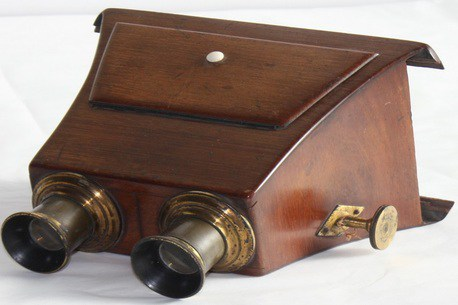
\includegraphics[scale = 0.5]{brewer.jpg}
\caption{Stéréoscope de Brewer.}
\end{figure}

Un procédé voisin mais néanmoins différent est celui de l'anaglyphe. Ce procédé sera décrit plus en détail dans la section 3.2 \ref{anasbs}.
Actuellement les dispositifs les plus populaires s'inspirent du stéréoscope de Brewer pour reconstruire le relief comme le fait l'Oculus Rift ou l'HTC Vive. La technologie side-by-side est utilisée ici et
sera vu en détail dans la section \ref{anasbs}.

Ces deux procédès ont très vite été adaptés aux vidéos afin de rendre les films plus vivants et réels et ainsi augmenter l'immersion.
A l'heure actuelle tous ces procédés utilisent 2 photographies ou vidéos prise avec un point de vue différents.  Le rendu du relief est alors très convaincant car très proche de la réalité.
Cependant, se procurer deux caméras ou appareils photos est très onéreux et n'est pas à la portée de tout le monde. Le but ici sera donc de réfléchir et de trouver un moyen de produire
cette stéréoscopie à partir d'une seule source vidéo ou d'une seule photographie tout en obtenant un relief le plus convaicant possible. Le résultat ne sera cependant jaais le même qu'avec deux images,
la perspective étant fixe à partir d'une seule source. Lors d'une prise avec 2 appareils, certains éléments sortent du cadre de la photo tandis que d'autred y entre. La quantité
d'informations présente sur une image est fixe. La translation qui se fera pour produire le décalage entre les deux yeux constituera alors une perte d'informations sans aucun gain.

Le but ici est donc d'automatiser le processus de création d'une vidéo stéréoscopique anaglyphe et side-by-side à partir d'une seule source vidéo tout ceci en JAVA.

\section{Laboratoire d'accueil}



\section{Etat de l'art et matériel existant}
\subsection{Résumé vidéo}
Le résumé vidéo peut aussi être appelé "Movie Barcode". Il permet de faire ressortir la couleur générale d'un film ou d'une vidéo. En récupérant la bande du milieu de chaque image et en concatenant tout cela pour
tout le film, on obtient une image très similaire à un code barre représentant l'ambiance générale de la vidéo.
Il existe un logiciel disponible réalisant ce traitement nommé "Movie Barcode Generator". Le logiciel est écrit en C\# et ses sources sont disponibles à tous. L'auteur du logiciel accepte la vente des
résultats produit par son logiciel.

\subsection{Anaglyphe et side-by-side}
\label{anasbs}
Actuellement, le vidéo 3D par anaglyphe propose deux méthodes majeures, un algorithme simple et la méthode de Dubois.
Le premier algorithme consiste à séparer et extraire les canaux RGB d'une image 2D et d'en faire une image 3D. Le principe réside dans le filtrage des couleurs par l'oeil devant lequel se trouve un filtre.
Chaque oeil ayant un filtre différent, il ne perçoit que les couleurs que le filtre laisse passer. Actuellement, le filtre le plus répandu est le filtre rouge/cyan.
Il suffit donc dans le cas de cet algortihme, d'extraire le canal rouge de l'image et d'en génerer un nouvelle. Ensuite il faut à partir de l'image source créer une nouvelle image à partir du mélange des canaux bleu et vert.
On obtient ainsi deux images, une cyan et l'autre rouge. Il faut ensuites les superposer en leur appliquant un décalage.\newline

La méthode de Dubois propose quant à elle de modifier les couleurs de l'image avant de lui appliquer l'algorithme vu précedemment.
En effet, afin de génerer des couleurs anaglyphe les plus proche possible de l'originale, Dubois tiens compte de la sensibilité spectrale de l'oeil humain,
le spectre d'absorption des filtre des lunettes et de la densité du spectre des moniteurs.
Dubois a alors pu en déduire une matrice à appliquer sur l'image originale permettant un effet 3D amélioré et la quasi
disparition des images fantômes qui sont des images résultat d'une supersition mal effectuée.
Le logiciel open-source Gimpel3D permet de faire de l'anaglyphe à partir d'images seulement et ne propose pas la méthode de Dubois. Nombre de logiciels payant existent et propose de réaliser des vidéos 3D
anaglyphe suivant l'algorithme basique comme par exemple DVDFab 9 ou  3D Video Converter.\newline

En ce qui concerne le side-by-side, le principe est de reproduire la distinction entre l'oeil droit et l'oeil gauche à travers une vidéo en comportant deux légérement décalés.
Il existe à l'heure actuelle beaucoup de logiciels qui proposent de faire ceci mais uniquement à partir de deux vidéos enregistrés préalablement avec le décalage.
Un seul logiciel exécute ce traitement avec une seule vidéo et il s'agit de DVDFab 9. Il est cependant payant et il n'existe aucun autre logiciel gratuit ou open-source réalisant ce traitement.

\subsection{Les flux vidéos en JAVA}

Très peu de bibliothèques manipulant des vidéos existent en JAVA. Au fil des recherches, la première bibliothèque que j'ai pu rencontrer est JAVACV, qui est un wrapper\footnote{Englobage d'un élément déjà existant
afin de simplifier son utilisation.} autour d'OpenCV. Cependant, les performances de JAVACV sont encore aujourd'hui sujet de débat.\\

J'ai donc préféré m'orienter vers des bibliothèques multimédias. J'ai trouvé par la suite la bibliothèque nommée Xuggler quiest un wrapper autour de
ffmpeg\footnote{Collection de logiciel libre permettant le traitement de flux audio et vidéos.} pour JAVA. Après quelques essais en ligne de commande de ce qui était offert
par ffmpeg (extraction des frames d'une vidéo, grands nombre de formats décodables,etc...), j'ai donc voulu essayer Xuggler. Malheureusment, cette bibliothèque n'est plus maintenue à jour, en effet le dernier
commit GitHub date de 2014. En recherchant d'autres wrapper autour de ffmpeg j'ai finalement pu tomber sur la bibliothèque OpenIMAJ et c'est celle-ci que j'utiliserais.\\

Afin de traiter les flux vidéos et de faire le traitement nécessaire sur les images tirées des vidéos, je me servirais de  la bibliothèque OpenImaj car multimédia, et maintenue à jour.
Cette bibliothèque présente de nombreux avantages. Tout d'abord elle est
disponible via un dépot Maven sous forme de modules. On peut donc récupérer uniquement les élèments de la bibliothèque
les plus pertinents. J'ai donc besoin ici des modules de décodage vidéo et de son, du module de traitemant d'images
et du module gérant les entrées/sorties.
Comme dit précedemment, OpenIMAJ est un wrapper ffmpeg. On aura donc l'avantage ici de pouvoir décoder les formats vidéos
les plus utilisés, causant alors très peu de problèmes de compatibilité dans notre
programme.\\

L'encodage quant à lui est par contre beaucoup plus restreint. Cela ne nous empêchera pas de produire
le fichier de sortie dans les formats les plus courants c'est-à-dire MP4, AVI ou MKV.
En ce qui concerne l'image, notre programme donnera en sortie une image au format PNG afin d'éviter la perte de donnée et
pour pouvoir l'exporter facilement sur le web.

Le son des vidéos sera quant à lui restitué tel qu'il l'était sur le fichier source.


\section{Cahier des charges et architecture}

Besoins fonctionnels :\newline
\begin{itemize}
\item S'affiche sous forme de fenêtre.
\item Choisir le fichier à traiter.
\item Préciser si la vidéo est décodable par le logiciel ou non. Si non, précisez les formats acceptés.
\item choix du mode de traitement et de l'algorithme (pour l'anaglyphe choisir entre l'agorithme classique ou la méthode
de Dubois).
\item Effectuer le traitement à l'aide d'un bouton.
\item Montrer l'avancement du traitement.
\item Sauvegarder le fichier sous le nom que l'on veut.
\item prévisualiser la vidéo séléctionnée\newline
\end{itemize}

Non fonctionnels :\newline
\begin{itemize}
\item Le logiciel doit être rapide. Le traitement doit s'effectuer dans le pire des cas dans le temps de la vidéo.
\item Fidélité. Le logiciel ne doit pas détériorer la qualité de la vidéo originelle.
pdf.\newline
\end{itemize}



\section{Implémentation}

La première chose que j'ai eu à réaliser a été de créer le projet Maven\footnote{Outil pour la gestion automatique des projets.}. OpenIMAJ étant disponible via Maven,
j'ai eu a rédiger le fichier pom.xml permettant de récupérer les modules nécessaires. Le fichier es découpé en section à l'aide de balises de façon similaire à l'HTML. Il faut en début de fichier,
déclarer le projet, sa version, ainsi que les dépots distants où récupérer les modules.

\begin{figure}[!h]
\center
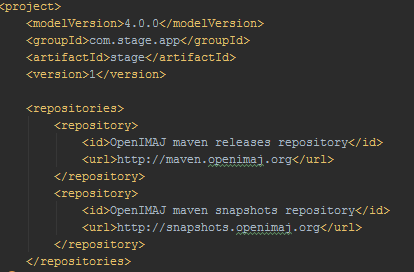
\includegraphics[scale = 1]{rapport.PNG}
\caption{En-tête du fichier pom.xml.}
\end{figure}

Il faut ensuite ouvrir la balise des dépendances et inscrire chaque dépendance que l'on trouve sur le site du dépot Maven de OpenIMAJ\footnote{https://mvnrepository.com/artifact/org.openimaj}.

\begin{figure}[h]
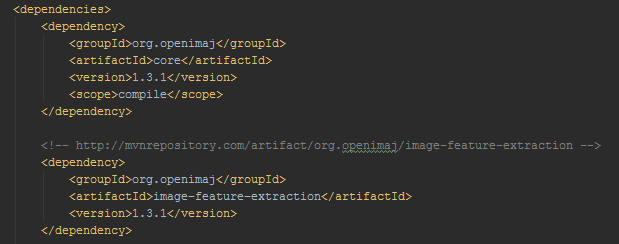
\includegraphics[scale = 1,inner]{dependance.PNG}
\caption{Inscription des dépendances.}
\end{figure}

Une fois ceci fait, j'ai organisé mon projet en créant tous les packages nécessaires c'est-à-dire : boutons, exceptions,traitements et utils.
A la racine de dossier src se trouve la classe Main me permettant d'initialiser l'interface et de lancer le programme. Un dossier resources est également présent comportant tous les fichiers
nécessaires pour les tests. J'ai également créé un dossier test et rajouter la dépendance JUnit dasn le fichier pom.xml pour effectuer les tests unitaires.

Tous les algoritmes seront contenus dans la classe Traitement et tout sera implementé en static y compris les données membres, les données membres étant le fichier de sortie et la vidéo.
Le programme n'ouvrant qu'une vidéo, il est plus simple de la mettre en static pour qu'elle ne dépende pas d'une instance et soit disponible pour tous les traitements.

\begin{figure}[!h]
\center
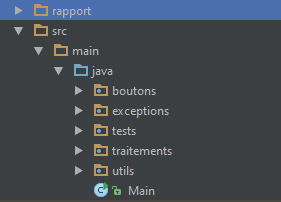
\includegraphics[scale = 1]{tree.PNG}
\caption{Arborescence du projet.}
\end{figure}

Je commence ensuite l'élaboration des algorithmes. J'ai donc commencé par l'écriture de l'algorithme du movie barcode.
\subsection{Movie Barcode}

Le movie barcode doit pour restaurer la couleur d'une image, récupérer la bande centrale de chaque frame de la vidéo. je suis donc passé par l'écriture de la méthode \textit{getBandeCentrale(MBFImage source)},
qui prends en paramètre une frame et retourne la bande centrale de cette frame. L'agortihme se place au milie de l'image et la parcours de la manière suivante : $milieu - tailleBande /2$ jusqu'à
$milieu + tailleBande /2$.\\
Ainsi j'ai pu obtenir la bande centrale de n'importe quelle image qui m'est retournée.

\begin{figure}[!h]
\center
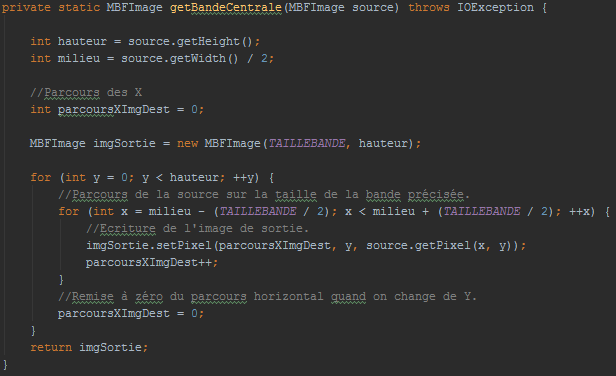
\includegraphics[scale = 1]{bandecentrale.png}
\caption{Méthode de récupération de la bande centrale.}
\end{figure}

Une fois ceci fait, l'algorithme du barcode se contente de concaténer toutes les bandes centrales dans une seule image finale. Le progrramme ne parcours cependant que les keyframes,
les keyframes étant les seules mages codées complétement dans une vidéo,
les autres étant calculées à partir des précédentes (P-frame) ou des suivantes (B-frame)\footnote{http://www.dacast.com/blog/what-is-a-key-frame-for-video/}.

INSERER SCREEN BARCODE.


\subsection{Anaglyphe}

L'algorithme d'anaglyphe récupère toutes les frames d'une vidéo et leur applique à chacune l'effet d'anaglyphe. Cela passe donc par la méthode \textit{anaglypheImage(MBFImage source, int largeur, int hauteur)}
qui récupère l'image en paramètre et retourne la même image anaglyphée. Le passage en paramètre de la hauter et de la largeur évite de recalculer ces deux données à chaque appel de la méthode.

\begin{figure}[!h]
\center
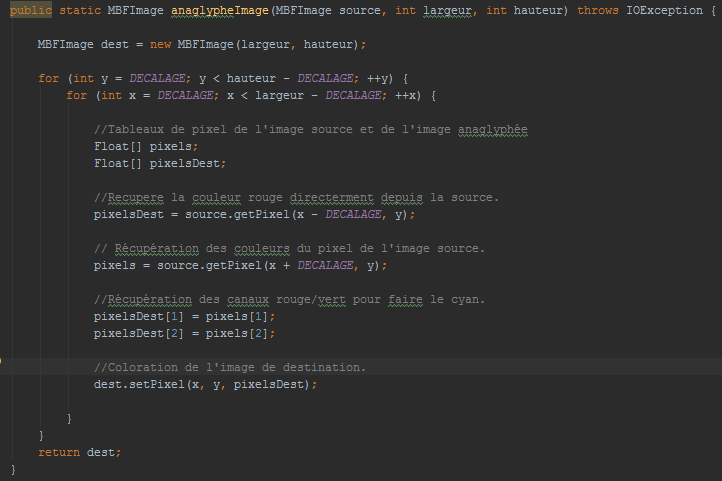
\includegraphics[scale = 1]{anaglypheimage.PNG}
\caption{Algorithme de création de l'effet anaglyphe.}
\end{figure}

l'algortihme créant la vidéo anaglyphée consiste à envoyer toutes les frames àa cette méthode et à reconstruire une vidéo à partir de ces frames à l'aide de l'objet
\textit{XuggleVideoWriter}. Le format de sortie de la vidéo est spécifié par le format d'entrée.

\subsection{side-by-side}



\section{Phase de test}

\section{Conclusion}

Josette CACHELOU, « STÉRÉOSCOPIE  », Encyclopædia Universalis [en ligne], consulté le 7 juillet 2016. URL : http://www.universalis.fr/encyclopedie/stereoscopie/

https://github.com/artclarke/xuggle-xuggler

https://github.com/bytedeco/javacv

http://www.xuggle.com/xuggler/

http://openimaj.org/

http://www.virtual-reality-shop.co.uk/brewster-stereoscope/
\end{document}
